\documentclass[10pt,a4paper,twocolumn]{article}
\usepackage[T1]{fontenc}
\usepackage[utf8]{inputenc}
\usepackage[french]{babel}
\usepackage{amsmath,amsthm,mathtools}
\usepackage{stix2}
\usepackage[scaled=0.95]{zi4}
\usepackage[a4paper,left=1.8cm,right=1.8cm,top=2.3cm,bottom=2.2cm,columnsep=0.6cm,headsep=0.45cm]{geometry}
\usepackage{microtype}
\usepackage{graphicx}
\usepackage{booktabs}
\usepackage{xcolor}
\usepackage[font=small,labelfont=sc,labelsep=period]{caption}
\usepackage{listings}
\usepackage{fancyhdr}
\usepackage{titlesec}
\usepackage{enumitem}
\usepackage[hidelinks]{hyperref}

\frenchsetup{StandardItemLabels=true}
\setlist{nosep,leftmargin=1.3em}
\addto\captionsfrench{%
  \renewcommand{\proofname}{Preuve}%
  \renewcommand{\figurename}{Fig.}%
  \renewcommand{\tablename}{Tab.}}

% ---------- en-tête et pied de page
\pagestyle{fancy}
\fancyhf{}
\fancyhead[C]{\small\itshape Modèle markovien d'une station Vélib'}
\fancyfoot[C]{\small\thepage}
\renewcommand{\headrulewidth}{0.4pt}

% ---------- titres
\titleformat{\section}{\normalfont\large\bfseries}{\thesection}{0.6em}{}
\titlespacing*{\section}{0pt}{9pt plus 2pt minus 2pt}{4pt plus 1pt}
\titleformat{\subsection}{\normalfont\normalsize\bfseries}{\thesubsection}{0.5em}{}
\titlespacing*{\subsection}{0pt}{6pt plus 2pt minus 1pt}{3pt plus 1pt}
\titleformat{\paragraph}[runin]{\normalfont\normalsize\bfseries}{}{0pt}{}[.]
\titlespacing*{\paragraph}{0pt}{3pt plus 1pt}{0.5em}

% ---------- énoncés
\newtheoremstyle{enonce}{3pt plus 1pt}{3pt plus 1pt}{\itshape}{}{\bfseries}{.}{0.4em}%
  {\thmname{#1}\thmnumber{ #2}\thmnote{ (\mdseries #3)}}
\newtheoremstyle{defi}{3pt plus 1pt}{3pt plus 1pt}{\normalfont}{}{\bfseries}{.}{0.4em}%
  {\thmname{#1}\thmnumber{ #2}\thmnote{ (\mdseries #3)}}
\theoremstyle{enonce}
\newtheorem{theoreme}{Théorème}[section]
\newtheorem{proposition}[theoreme]{Proposition}
\newtheorem{lemme}[theoreme]{Lemme}
\newtheorem{corollaire}[theoreme]{Corollaire}
\theoremstyle{defi}
\newtheorem{definition}[theoreme]{Définition}
\newtheorem{remarque}[theoreme]{Remarque}

% ---------- code
\definecolor{vertTIPE}{RGB}{24,110,83}
\definecolor{grisCode}{RGB}{105,110,120}
\lstdefinestyle{py}{language=Python, basicstyle=\ttfamily\scriptsize,
  keywordstyle=\color{vertTIPE}\bfseries, commentstyle=\color{grisCode}\itshape,
  stringstyle=\color{grisCode}, showstringspaces=false, columns=fullflexible,
  keepspaces=true, frame=lines, framerule=0.3pt, rulecolor=\color{grisCode},
  aboveskip=3pt, belowskip=1pt, breaklines=true}

% ---------- notations
\newcommand{\PP}{\mathbb{P}}
\newcommand{\EE}{\mathbb{E}}
\newcommand{\VT}{\mathrm{VT}}
\newcommand{\dd}{\mathrm{d}}
\newcommand{\un}{\mathbf{1}}
\newcommand{\hr}{\,\mathrm{h}^{-1}}
\newcommand{\trel}{t_{\mathrm{rel}}}
\newcommand{\tmel}{t_{\mathrm{m\acute el}}}
\newcommand{\Nu}{N^{\uparrow}}
\newcommand{\Nd}{N^{\downarrow}}
\newcommand{\Tu}{T^{\uparrow}}
\newcommand{\Td}{T^{\downarrow}}

\begin{document}

\twocolumn[{%
\begin{center}
{\LARGE\bfseries Modèle markovien d'une station Vélib'~:\\[3pt]
régime stationnaire, calibration et limites\par}
\vspace{9pt}
{\large Matthias Nguyen\par}
\vspace{3pt}
{\small Lycée Sainte-Geneviève, Versailles\par}
% {\small\ttfamily adresse électronique\par}
\vspace{2pt}
{\small Novembre 2026\par}
\end{center}
\vspace{2pt}
\begin{center}
\begin{minipage}{0.9\textwidth}
\begin{center}\textbf{Abstract}\end{center}
\vspace{-5pt}
\small\selectlanguage{english}
We model the number of bikes at a bike-sharing station as a continuous-time birth--death chain on $\{0,\dots,C\}$, that is, an M/M/1/C queue. We give a self-contained treatment of the tools involved: existence, uniqueness and geometric convergence of the stationary law through a Doeblin contraction argument, the full spectrum of the generator with two-sided bounds on the distance to equilibrium, and closed-form hitting times. Rates are estimated by maximum likelihood from minute-by-minute records of Paris stations (May--June 2026). Likelihood-ratio tests reject constant rates within a day ($p<10^{-27}$). With rates constant on two-hour slots, out-of-sample 90\,\% prediction bands cover 88\,\% of observed minutes at a two-hour horizon. The stationary law is never observed: mixing times (5 to 48 hours) exceed the time scale on which rates change. The relevant object is the periodic regime of the inhomogeneous chain, which forgets its initial state by a factor 0.13 per day. We also show that two numerical shortcuts of a preliminary study lowered its midday forecast by 16 bikes. The same framework underlies queue-based models of limit order books and generator estimation in credit risk.

\smallskip
\noindent\textit{Keywords:} continuous-time Markov chains, birth--death processes, spectral gap, maximum likelihood, backtesting, bike sharing, limit order books.
\selectlanguage{french}
\end{minipage}
\end{center}
\vspace{10pt}
}]
{\renewcommand{\thefootnote}{}\footnotetext{Ce texte reprend et prolonge la partie personnelle d'un TIPE de mathématiques préparé en classe de MP* (session 2026), désigné ci-dessous par \og le TIPE\fg{}.}}

\section{Introduction}\label{sec:intro}

Une station Vélib' de $C$ bornes alterne des phases où elle se vide et des phases où elle se remplit. Vide, elle refuse les retraits~; pleine, elle refuse les dépôts. L'opérateur corrige ces déséquilibres par camions. Prévoir l'occupation d'une station à quelques heures conditionne donc les tournées de régulation et le dimensionnement des stations.

Le modèle le plus simple décrit le nombre de vélos $X_t$ comme une chaîne de Markov à temps continu de naissance et de mort, bornée par $0$ et $C$~: c'est la file M/M/1/C \cite{STGH18}. Raviv et Kolka \cite{RK13} l'utilisent avec des taux dépendant du temps pour définir une fonction d'insatisfaction des usagers. Schuijbroek, Hampshire et van Hoeve \cite{SHH17} en déduisent des niveaux de service qui contraignent la planification de la régulation. Fricker et Gast \cite{FG16} étudient la limite de champ moyen d'un réseau homogène de telles stations.

La même structure apparaît en microstructure des marchés. La file d'ordres à un niveau de prix est un processus de naissance et de mort, alimenté par les ordres limites et vidé par les ordres au marché et les annulations \cite{CST10,CdL13,HLR15}. L'estimation d'un générateur à partir de trajectoires observées en continu est aussi celle des matrices de migration de notations en risque de crédit \cite{JLT97,LS02}. La section~\ref{sec:discussion} revient sur ces analogies.

\paragraph{Contributions} (i) Un exposé autonome des outils~: convergence vers la loi stationnaire par contraction de Doeblin, spectre explicite du générateur, bornes de convergence et temps d'atteinte. (ii) Une estimation par maximum de vraisemblance avec temps d'exposition, intervalles de confiance et tests du rapport de vraisemblance. (iii) Une validation hors échantillon à 2~h et à 24~h sur des relevés minute par minute de deux stations parisiennes. (iv) Une explication quantitative de l'échec de la loi stationnaire~: les temps de mélange dépassent l'échelle de variation des taux, et l'objet pertinent est le régime périodique de la chaîne inhomogène. (v) La correction de deux biais numériques de l'étude préliminaire.

La section~\ref{sec:outils} rassemble les outils probabilistes, la section~\ref{sec:modele} étudie le modèle à taux constants, les sections~\ref{sec:estimation} et~\ref{sec:simulation} traitent l'estimation et la simulation. La section~\ref{sec:resultats} confronte le modèle aux données et la section~\ref{sec:discussion} discute ses limites. Le code figure en annexe~\ref{sec:code}.

\section{Outils probabilistes}\label{sec:outils}

Cette section fixe le cadre. Les résultats de théorie de la mesure utilisés (unicité des mesures, Fubini--Tonelli, changement de variable) sont admis \cite{JP04}.

\subsection{Variables aléatoires et lois}

\begin{definition}
Une \emph{tribu} sur un ensemble $\Omega$ est une partie $\mathcal{F}\subset\mathcal{P}(\Omega)$ qui contient $\Omega$ et qui est stable par passage au complémentaire et par union dénombrable. Une \emph{probabilité} sur $(\Omega,\mathcal{F})$ est une application $\PP:\mathcal{F}\to[0,1]$ telle que $\PP(\Omega)=1$ et $\PP\big(\bigcup_{n\geq1}A_n\big)=\sum_{n\geq1}\PP(A_n)$ pour toute suite $(A_n)_{n\geq1}$ d'éléments de $\mathcal{F}$ deux à deux disjoints. Le triplet $(\Omega,\mathcal{F},\PP)$ est un \emph{espace probabilisé}~; les éléments de $\mathcal{F}$ sont les \emph{événements}.
\end{definition}

\begin{definition}
Soient $(E,\mathcal{E})$ et $(E',\mathcal{E}')$ deux espaces mesurables. Une application $f:E\to E'$ est \emph{mesurable} si $f^{-1}(B)\in\mathcal{E}$ pour tout $B\in\mathcal{E}'$. Une \emph{variable aléatoire} à valeurs dans $(E',\mathcal{E}')$ est une application mesurable $X:(\Omega,\mathcal{F})\to(E',\mathcal{E}')$. Sa \emph{loi} est la mesure image $\PP_X$ définie par $\PP_X(B)=\PP(X^{-1}(B))=\PP(X\in B)$ pour $B\in\mathcal{E}'$.
\end{definition}

On munit $\mathbb{R}$ de la tribu borélienne $\mathcal{B}(\mathbb{R})$, engendrée par les intervalles $]-\infty,t]$, et un ensemble fini $E$ de la tribu $\mathcal{P}(E)$. Comme $\{B:X^{-1}(B)\in\mathcal{F}\}$ est une tribu, une application $X:\Omega\to\mathbb{R}$ est une variable aléatoire dès que $\{X\leq t\}\in\mathcal{F}$ pour tout réel $t$. Sommes, produits, limites simples de variables aléatoires réelles et composées par des fonctions boréliennes sont des variables aléatoires. La loi d'une variable à valeurs dans $E$ fini est le vecteur $\big(\PP(X=i)\big)_{i\in E}$.

\begin{definition}
La \emph{fonction de répartition} d'une variable aléatoire réelle $X$ est $F_X(t)=\PP(X\leq t)$, $t\in\mathbb{R}$. Une fonction borélienne $f\geq0$ telle que $\int_{\mathbb{R}}f(x)\,\dd x=1$ est une \emph{densité} de $X$ si $\PP(X\in B)=\int_Bf(x)\,\dd x$ pour tout $B\in\mathcal{B}(\mathbb{R})$.
\end{definition}

Par continuité monotone de $\PP$, $F_X$ est croissante et continue à droite. Elle caractérise la loi~: deux probabilités qui coïncident sur les intervalles $]-\infty,t]$, famille stable par intersection finie qui engendre $\mathcal{B}(\mathbb{R})$, coïncident sur $\mathcal{B}(\mathbb{R})$ (lemme de classe monotone). L'espérance d'une variable aléatoire $X$ positive ou intégrable est $\EE[X]=\int_\Omega X\,\dd\PP$. Si $X$ a pour densité $f$ et si $g$ est borélienne positive, ou telle que $g(X)$ soit intégrable, alors $\EE[g(X)]=\int_{\mathbb{R}}g(x)f(x)\,\dd x$ (théorème de transfert).

\begin{definition}
Des sous-tribus $\mathcal{G}_1,\dots,\mathcal{G}_m$ de $\mathcal{F}$ sont \emph{indépendantes} si $\PP(A_1\cap\dots\cap A_m)=\prod_{k=1}^m\PP(A_k)$ pour tous $A_1\in\mathcal{G}_1,\dots,A_m\in\mathcal{G}_m$. Des variables aléatoires $X_1,\dots,X_m$, à valeurs dans des espaces $(E_k,\mathcal{E}_k)$, sont indépendantes si les tribus $\sigma(X_k)=\{X_k^{-1}(B):B\in\mathcal{E}_k\}$ le sont~; une suite de variables est indépendante si toute sous-famille finie l'est.
\end{definition}

Des variables réelles $X_1,\dots,X_m$ de densités $f_1,\dots,f_m$ sont indépendantes si et seulement si le vecteur $(X_1,\dots,X_m)$ a pour densité $(x_1,\dots,x_m)\mapsto\prod_{k=1}^mf_k(x_k)$ sur $\mathbb{R}^m$. Les probabilités qui le concernent se calculent alors par le théorème de Fubini--Tonelli. En particulier, si $X$ et $Y$ sont indépendantes de densités $f$ et $g$, alors pour $B\in\mathcal{B}(\mathbb{R})$, avec le changement de variable $z=x+y$,
\begin{align*}
\PP(X+Y\in B)&=\int_{\mathbb{R}^2}\un_B(x+y)f(x)g(y)\,\dd x\,\dd y\\
&=\int_B(f*g)(z)\,\dd z,
\end{align*}
où $(f*g)(z)=\int_{\mathbb{R}}f(x)g(z-x)\,\dd x$~: la somme $X+Y$ a pour densité $f*g$. Enfin, des fonctions mesurables de paquets disjoints de variables indépendantes sont indépendantes (regroupement par paquets).

\subsection{Loi exponentielle}

\begin{definition}
Une variable aléatoire réelle $T$ suit la loi exponentielle $\mathcal{E}(a)$, $a>0$, si elle a pour densité $x\mapsto ae^{-ax}\un_{\{x\geq0\}}$. Alors $\PP(T>t)=e^{-at}$ pour $t\geq0$, $\EE[T]=1/a$ et $\mathrm{Var}(T)=1/a^2$.
\end{definition}

\begin{proposition}[absence de mémoire]\label{prop:memoire}
Soit $T$ une variable aléatoire réelle telle que $\PP(T>0)=1$. Les assertions suivantes sont équivalentes~:
\begin{enumerate}[label=(\roman*)]
\item $\PP(T>s+t)=\PP(T>s)\,\PP(T>t)$ pour tous $s,t\geq0$~;
\item $T$ suit une loi exponentielle.
\end{enumerate}
\end{proposition}

\begin{proof}
(ii)~$\Rightarrow$~(i) est immédiat. Réciproquement, posons $G(t)=\PP(T>t)=1-F_T(t)$. Par continuité monotone de $\PP$, $G$ est décroissante, continue à droite, $G(0)=1$ et $G(t)\to0$ quand $t\to+\infty$. Si $G(1)=0$, alors $G(1/n)^n=G(1)=0$, donc $G(1/n)=0$ pour tout $n\geq1$, ce qui contredit $G(1/n)\to G(0)=1$. Si $G(1)=1$, alors $G(n)=G(1)^n=1$ pour tout $n$, ce qui contredit $G\to0$. Donc $G(1)=e^{-a}$ avec $a>0$. L'équation fonctionnelle donne $G(1/q)=e^{-a/q}$, puis $G(p/q)=e^{-ap/q}$ pour $p,q\in\mathbb{N}^*$, et la décroissance de $G$ étend l'égalité à tout réel $t\geq0$. Comme $F_T(t)=0$ pour $t<0$, $F_T$ est la fonction de répartition de $\mathcal{E}(a)$, qui caractérise la loi.
\end{proof}

\begin{lemme}[horloges en compétition]\label{lem:horloges}
Soient $A_1,\dots,A_m$ des variables aléatoires indépendantes, $A_i\sim\mathcal{E}(a_i)$, et $a=\sum_{i=1}^ma_i$. Presque sûrement, le minimum $M=\min_iA_i$ est atteint en un unique indice $I$. On a $M\sim\mathcal{E}(a)$, $\PP(I=i)=a_i/a$, et $M$ et $I$ sont indépendants.
\end{lemme}

\begin{proof}
Pour $i\neq j$, le couple $(A_i,A_j)$ a une densité sur $\mathbb{R}^2$ et la diagonale est de mesure de Lebesgue nulle, donc $\PP(A_i=A_j)=0$. L'indice $I$ est ainsi défini presque sûrement, et $\{I=i\}=\bigcap_{j\neq i}\{A_j>A_i\}$ est un événement. Le vecteur $(A_1,\dots,A_m)$ a pour densité le produit des densités~; pour $t\geq0$, le théorème de Fubini--Tonelli donne
\begin{align*}
\PP(M>t,\,I=i)&=\int_t^{+\infty}a_ie^{-a_is}\prod_{j\neq i}\PP(A_j>s)\,\dd s\\
&=\frac{a_i}{a}\,e^{-at}.
\end{align*}
La somme sur $i$ donne $\PP(M>t)=e^{-at}$, le cas $t=0$ donne $\PP(I=i)=a_i/a$. La factorisation $\PP(M>t,I=i)=\PP(M>t)\PP(I=i)$ s'étend à $\sigma(M)$ par classe monotone~: $M$ et $I$ sont indépendants.
\end{proof}

\subsection{Processus de Poisson}

\begin{definition}
Soient $(\tau_k)_{k\geq1}$ des variables aléatoires indépendantes de loi $\mathcal{E}(\lambda)$, $S_0=0$ et $S_n=\sum_{k=1}^n\tau_k$. Le \emph{processus de Poisson} d'intensité $\lambda$ est la famille $(N_t)_{t\geq0}$ définie par $N_t=\sum_{n\geq1}\un_{\{S_n\leq t\}}$.
\end{definition}

Chaque $N_t$ est une variable aléatoire à valeurs dans $\mathbb{N}\cup\{+\infty\}$, limite croissante de variables aléatoires. Elle est finie presque sûrement~: par indépendance, $\EE[e^{-S_n}]=\big(\lambda/(1+\lambda)\big)^n$, et par convergence dominée $\EE\big[\lim_ne^{-S_n}\big]=0$, donc $S_n\to+\infty$ presque sûrement.

\begin{proposition}\label{prop:poisson}
$S_n$ a pour densité $f_n(s)=\lambda^ns^{n-1}e^{-\lambda s}\un_{\{s>0\}}/(n-1)!$, et pour tout $t>0$, $N_t$ suit la loi de Poisson de paramètre $\lambda t$.
\end{proposition}

\begin{proof}
Par regroupement par paquets, $S_n$ est indépendante de $\tau_{n+1}$. Si $S_n$ a pour densité $f_n$, la variable $S_{n+1}=S_n+\tau_{n+1}$ a donc pour densité
\[
(f_n*f_1)(s)=\int_0^s\frac{\lambda^nx^{n-1}e^{-\lambda x}}{(n-1)!}\,\lambda e^{-\lambda(s-x)}\,\dd x=f_{n+1}(s)
\]
pour $s>0$, d'où la première assertion par récurrence. On vérifie que $\frac{\dd}{\dd t}\big(e^{-\lambda t}(\lambda t)^n/n!\big)=f_n(t)-f_{n+1}(t)$ pour $n\geq1$. Comme $(S_n)$ est croissante, $\{N_t\geq n\}=\{S_n\leq t\}$, et
\[
\PP(N_t=n)=\PP(S_n\leq t)-\PP(S_{n+1}\leq t)=e^{-\lambda t}\frac{(\lambda t)^n}{n!},
\]
avec $\PP(N_t=0)=\PP(\tau_1>t)=e^{-\lambda t}$.
\end{proof}

Le processus $(N_t)$ est de plus à accroissements indépendants et stationnaires \cite[§2.4]{Nor97}.

\begin{remarque}\label{rem:palm}
La superposition d'un grand nombre de flux indépendants, chacun de faible intensité, est approximativement poissonnienne (théorème de Palm--Khintchine \cite{DVJ03}). C'est la justification usuelle de l'hypothèse poissonnienne pour les usagers d'une station. La section~\ref{sec:poisson} en teste les limites.
\end{remarque}

\subsection{Chaînes de Markov à temps continu}

Soit $E$ un ensemble fini, muni de la tribu $\mathcal{P}(E)$. Un \emph{processus} à valeurs dans $E$ est une famille $(X_t)_{t\geq0}$ de variables aléatoires à valeurs dans $E$. Une matrice $Q=(q_{ij})_{i,j\in E}$ est un \emph{générateur} si $q_{ij}\geq0$ pour $i\neq j$ et $\sum_{j\in E}q_{ij}=0$ pour tout $i$. On note $q_i=-q_{ii}=\sum_{j\neq i}q_{ij}$ et $\bar q=\max_iq_i$.

\begin{definition}
Soit $(P(t))_{t\geq0}$ une famille de matrices stochastiques. Un processus $(X_t)_{t\geq0}$ est une \emph{chaîne de Markov homogène} de semi-groupe $(P(t))$ si pour tous $0\leq t_0<\dots<t_n<t$ et $i_0,\dots,i_n,j\in E$ tels que $\PP(X_{t_0}=i_0,\dots,X_{t_n}=i_n)>0$,
\[
\PP(X_t=j\mid X_{t_0}=i_0,\dots,X_{t_n}=i_n)=P(t-t_n)_{i_nj}.
\]
On note $\PP_i$ la probabilité conditionnelle sachant $X_0=i$ et $\EE_i$ l'espérance associée.
\end{definition}

Comme $E$ est fini, conditionner par des événements de probabilité positive suffit.

\paragraph{Construction par sauts} Soient $(Y_n)_{n\geq0}$ une chaîne de Markov à temps discret sur $E$, de matrice de transition $\Pi$ donnée par $\Pi_{ij}=q_{ij}/q_i$ pour $j\neq i$ (et $\Pi_{ii}=1$ si $q_i=0$), et $(\varepsilon_n)_{n\geq1}$ des variables indépendantes de loi $\mathcal{E}(1)$, indépendantes de $(Y_n)$. On pose $J_0=0$, $J_{n+1}=J_n+\varepsilon_{n+1}/q_{Y_n}$ (avec $J_{n+1}=+\infty$ si $q_{Y_n}=0$), et $X_t=Y_n$ pour $J_n\leq t<J_{n+1}$. Sachant $Y_n=i$, la durée de séjour $J_{n+1}-J_n$ suit la loi $\mathcal{E}(q_i)$. Comme $J_n\geq(\varepsilon_1+\dots+\varepsilon_n)/\bar q$, $J_n\to+\infty$ presque sûrement, comme pour le processus de Poisson, et $X_t$ est défini pour tout $t$. D'après le lemme~\ref{lem:horloges}, on obtient la même loi en lançant dans l'état $i$ des horloges indépendantes de lois $\mathcal{E}(q_{ij})$, $j\neq i$~: la première qui sonne fixe l'instant et la destination du saut. C'est l'algorithme de simulation de la section~\ref{sec:simulation}.

\begin{proposition}[semi-groupe]\label{prop:semigroupe}
Le processus ainsi construit est une chaîne de Markov homogène de semi-groupe $P(t)=e^{tQ}=\sum_{k\geq0}t^kQ^k/k!$. Ce semi-groupe vérifie $P(s+t)=P(s)P(t)$ (Chapman--Kolmogorov) et $P'(t)=QP(t)=P(t)Q$ (équations de Kolmogorov). La loi $p(t)$ de $X_t$, vue comme vecteur ligne, vérifie $p(t)=p(0)\,e^{tQ}$.
\end{proposition}

Ce résultat est admis \cite[§2.6--2.8]{Nor97}, \cite{Guy07}~; la propriété de Markov y découle de l'absence de mémoire des durées de séjour. La représentation suivante de $e^{tQ}$ servira plusieurs fois.

\begin{lemme}[uniformisation]\label{lem:unif}
Soient $\Lambda>\max_iq_i$ et $K=I+Q/\Lambda$. La matrice $K$ est stochastique, de diagonale strictement positive, et
\begin{equation}\label{eq:unif}
e^{tQ}=\sum_{k\geq0}e^{-\Lambda t}\frac{(\Lambda t)^k}{k!}\,K^k.
\end{equation}
\end{lemme}

\begin{proof}
$K_{ij}=q_{ij}/\Lambda\geq0$ pour $i\neq j$, $K_{ii}=1-q_i/\Lambda>0$, et les lignes de $K$ somment à $1$. Comme $tQ=\Lambda t(K-I)$ et que $I$ et $K$ commutent, $e^{tQ}=e^{-\Lambda t}e^{\Lambda tK}$.
\end{proof}

La formule~\eqref{eq:unif} décrit une horloge de Poisson d'intensité $\Lambda$~; à chaque sonnerie, la chaîne saute selon $K$, éventuellement sur place.

\begin{definition}
$Q$ est \emph{irréductible} si pour tous $i\neq j$ il existe des états $i=i_0,i_1,\dots,i_r=j$ tels que $q_{i_{\ell-1}i_\ell}>0$ pour $1\leq\ell\leq r$.
\end{definition}

\begin{lemme}\label{lem:positif}
Si $Q$ est irréductible, $P(t)_{ij}>0$ pour tous $i,j\in E$ et $t>0$.
\end{lemme}

\begin{proof}
Avec un chemin de $i$ à $j$ comme ci-dessus, $(K^r)_{ij}\geq K_{i_0i_1}\cdots K_{i_{r-1}i_r}>0$, et $(K^0)_{ii}=1$. Le terme d'indice $r$ de~\eqref{eq:unif} est donc strictement positif.
\end{proof}

\subsection{Loi stationnaire et convergence}

\begin{definition}
Une loi $\pi$ sur $E$ est \emph{stationnaire} si $\pi Q=0$, c'est-à-dire si $\pi P(t)=\pi$ pour tout $t\geq0$. La distance en variation totale entre deux lois est
\[
\|\mu-\nu\|_\VT=\frac12\sum_{j\in E}|\mu_j-\nu_j|=\max_{A\subset E}|\mu(A)-\nu(A)|.
\]
\end{definition}

\begin{lemme}[Doeblin]\label{lem:doeblin}
Soient $P$ une matrice stochastique et $\delta(P)=\sum_{j\in E}\min_{i\in E}P_{ij}$. Pour toutes lois $\mu$ et $\nu$,
\[
\|\mu P-\nu P\|_\VT\leq\big(1-\delta(P)\big)\,\|\mu-\nu\|_\VT.
\]
\end{lemme}

\begin{proof}
Notons $m_j=\min_iP_{ij}$ et $\delta=\delta(P)$. Si $\delta=1$, toutes les lignes de $P$ valent $m$ et $\mu P=\nu P$. Sinon, $R=(P-\un m)/(1-\delta)$ est stochastique, où $\un$ est le vecteur colonne de uns. Comme $(\mu-\nu)\un=0$, on a $\mu P-\nu P=(1-\delta)(\mu-\nu)R$. Enfin, pour tout vecteur ligne $x$, $\sum_j|(xR)_j|\leq\sum_j\sum_i|x_i|R_{ij}=\sum_i|x_i|$.
\end{proof}

\begin{theoreme}[loi stationnaire]\label{thm:stationnaire}
Soient $Q$ un générateur irréductible sur $E$ fini et $h>0$. Il existe une unique loi stationnaire $\pi$~; elle charge tous les états. Pour toute loi initiale $\mu$ et tout $t\geq0$,
\[
\|\mu e^{tQ}-\pi\|_\VT\leq(1-\delta_h)^{\lfloor t/h\rfloor},\qquad \delta_h=\delta(e^{hQ})>0.
\]
\end{theoreme}

\begin{proof}
D'après le lemme~\ref{lem:positif}, $P(h)$ est à coefficients strictement positifs, donc $\delta_h>0$. L'ensemble $\mathcal{P}$ des lois sur $E$ est un fermé de $\mathbb{R}^E$, donc complet pour $\|\cdot\|_\VT$, et $\mu\mapsto\mu P(h)$ est une contraction de rapport $1-\delta_h$ sur $\mathcal{P}$ (lemme~\ref{lem:doeblin}). Le théorème du point fixe donne une unique loi $\pi$ telle que $\pi P(h)=\pi$. Pour $s\geq0$, $\pi P(s)$ est encore un point fixe, car $\pi P(s)P(h)=\pi P(h)P(s)=\pi P(s)$~; donc $\pi P(s)=\pi$ et $\pi$ est stationnaire. Une loi stationnaire est un point fixe, d'où l'unicité. Comme $\pi=\pi P(h)$ et $P(h)>0$, $\pi_j>0$ pour tout $j$. Enfin, pour $t=nh+r$ avec $0\leq r<h$,
\[
\|\mu P(t)-\pi\|_\VT=\|\mu P(r)P(h)^n-\pi P(h)^n\|_\VT\leq(1-\delta_h)^n.\qedhere
\]
\end{proof}

Le TIPE admettait ce résultat en invoquant le théorème de Perron--Frobenius. La preuve ci-dessus est autonome, mais la constante $1-\delta_h$ est en général très pessimiste~; la section~\ref{sec:spectre} donne la vitesse exacte pour notre modèle.

\begin{theoreme}[ergodique, admis {\cite[§3.8]{Nor97}}]\label{thm:ergodique}
Sous les hypothèses du théorème~\ref{thm:stationnaire}, pour toute fonction $f:E\to\mathbb{R}$ et toute loi initiale,
\[
\frac1t\int_0^tf(X_s)\,\dd s\xrightarrow[t\to+\infty]{\text{p.s.}}\sum_{j\in E}\pi_jf(j).
\]
\end{theoreme}

Avec $f=\un_{\{j\}}$, $\pi_j$ est la fraction du temps passée en $j$ sur le long terme. C'est en ce sens que la section~\ref{sec:nonstationnaire} confronte $\pi$ aux données.

\subsection{Taux constants par morceaux}\label{sec:periodique}

Soient $0=\tau_0<\tau_1<\dots<\tau_K=T$ et des générateurs $Q_1,\dots,Q_K$. La chaîne de générateur $Q_k$ sur $[\tau_{k-1},\tau_k[$ s'obtient en enchaînant les constructions par sauts~: arrivée en $\tau_{k-1}$ dans l'état $i$, elle repart de $i$ avec le générateur $Q_k$. C'est licite par absence de mémoire. La loi de $X_T$ vaut $p(T)=p(0)M$ avec
\[
M=e^{h_1Q_1}e^{h_2Q_2}\cdots e^{h_KQ_K},\qquad h_k=\tau_k-\tau_{k-1}.
\]
On prolonge les taux par $T$-périodicité, avec $T$ égal à un jour.

\begin{proposition}[régime périodique]\label{prop:periodique}
Supposons qu'au moins un $Q_k$ soit irréductible. Alors $M$ est à coefficients strictement positifs, $(X_{nT})_{n\geq0}$ est une chaîne de Markov homogène de matrice de transition $M$, et il existe une unique loi $\nu$ telle que $\nu M=\nu$. Pour toute loi initiale $\mu$ et tout $n\geq0$, $\|\mu M^n-\nu\|_\VT\leq(1-\delta(M))^n$. Pour $s\in[\tau_{k-1},\tau_k[$, la loi de $X_{nT+s}$ converge vers
\[
\nu_s=\nu\,e^{h_1Q_1}\cdots e^{h_{k-1}Q_{k-1}}e^{(s-\tau_{k-1})Q_k}.
\]
\end{proposition}

\begin{proof}
Chaque facteur $e^{h_kQ_k}$ est stochastique et de diagonale strictement positive, car $(e^{hQ})_{jj}\geq e^{-q_jh}$~; le facteur irréductible est strictement positif (lemme~\ref{lem:positif}). Si $A>0$ et si $B$ est stochastique de diagonale strictement positive, $(AB)_{ij}\geq A_{ij}B_{jj}>0$ et $(BA)_{ij}\geq B_{ii}A_{ij}>0$~; donc $M>0$. La propriété de Markov aux instants $nT$, où les taux recommencent le même cycle, donne la chaîne de matrice $M$. On conclut comme pour le théorème~\ref{thm:stationnaire}~; la convergence de $X_{nT+s}$ s'obtient en appliquant une matrice stochastique, qui contracte $\|\cdot\|_\VT$.
\end{proof}

La vitesse asymptotique d'oubli de l'état initial est le module $|\lambda_2(M)|$ de la deuxième plus grande valeur propre de $M$~; $1-\delta(M)$ en est une majoration.

\section{Modèle de station}\label{sec:modele}

\subsection{Hypothèses}

Soit $X_t\in E=\{0,\dots,C\}$ le nombre de vélos disponibles, mécaniques et électriques, dans une station de $C$ bornes.
\begin{enumerate}[label=(H\arabic*)]
\item Les usagers qui veulent déposer un vélo arrivent selon un processus de Poisson d'intensité $\lambda$~; ceux qui veulent en retirer un, selon un processus de Poisson d'intensité $\mu$, indépendant du premier.
\item Un dépôt dans une station pleine et un retrait dans une station vide sont perdus.
\item Les taux $\lambda$ et $\mu$ sont constants.
\end{enumerate}
L'hypothèse (H3) est relâchée en section~\ref{sec:resultats}, où les taux sont constants par créneaux de 2~h. Sous ces hypothèses, $X$ est la chaîne de générateur
\[
Q=\begin{pmatrix}
-\lambda & \lambda & & & \\
\mu & -(\lambda+\mu) & \lambda & & \\
 & \ddots & \ddots & \ddots & \\
 & & \mu & -(\lambda+\mu) & \lambda\\
 & & & \mu & -\mu
\end{pmatrix},
\]
c'est-à-dire $q_{n,n+1}=\lambda$ pour $n<C$ et $q_{n,n-1}=\mu$ pour $n>0$. C'est la file M/M/1/C~: les vélos jouent le rôle des clients, les retraits celui du service \cite[§3.5]{STGH18}, \cite{Bre99}. On note $\rho=\lambda/\mu$~; $Q$ est irréductible dès que $\lambda,\mu>0$.

\subsection{Loi stationnaire}

\begin{proposition}\label{prop:pi}
Pour $\lambda,\mu>0$, la loi stationnaire est
\[
\pi_n=\frac{\rho^n(1-\rho)}{1-\rho^{C+1}}\ \ (\rho\neq1),\qquad\pi_n=\frac{1}{C+1}\ \ (\rho=1).
\]
\end{proposition}

\begin{proof}
Cette loi vérifie l'équilibre détaillé $\pi_n\lambda=\pi_{n+1}\mu$ pour $0\leq n<C$. Notons $\phi_n=\pi_n\lambda-\pi_{n+1}\mu$ le flux net de $n$ vers $n+1$, avec $\phi_{-1}=\phi_C=0$. Alors $(\pi Q)_n=\phi_{n-1}-\phi_n=0$ pour tout $n$. On conclut par le théorème~\ref{thm:stationnaire}.
\end{proof}

\begin{corollaire}[indicateurs de service]\label{cor:indicateurs}
Sous $\pi$~:
\begin{enumerate}[label=(\roman*)]
\item la station est vide une fraction $\pi_0$ du temps et pleine une fraction $\pi_C$~;
\item les fractions de retraits et de dépôts refusés valent $\pi_0$ et $\pi_C$~;
\item $\EE_\pi[X]=\dfrac{\rho}{1-\rho}-\dfrac{(C+1)\rho^{C+1}}{1-\rho^{C+1}}$ si $\rho\neq1$, et $C/2$ si $\rho=1$~;
\item quand $C\to+\infty$, $\pi_0\to(1-\rho)^+$ et $\pi_C\to(1-1/\rho)^+$.
\end{enumerate}
\end{corollaire}

\begin{proof}
(i) est le théorème~\ref{thm:ergodique}. (ii) Les dépôts forment un processus de Poisson indépendant du passé de $X$~: un dépôt voit donc la station dans l'état moyen en temps, soit $\pi$ sur le long terme (propriété PASTA \cite{Wol82}). (iii) On écrit $\sum_{n=0}^Cn\rho^n=\rho\frac{\dd}{\dd\rho}\frac{1-\rho^{C+1}}{1-\rho}$ et on simplifie. (iv) Si $\rho<1$, $\rho^{C+1}\to0$~; si $\rho>1$, $\pi_C=\rho^C(\rho-1)/(\rho^{C+1}-1)\to1-1/\rho$.
\end{proof}

La loi $\pi$ est géométrique de raison $\rho$~: elle se concentre près de $0$ si $\rho<1$ et près de $C$ si $\rho>1$. D'après (iv), un déséquilibre $\rho>1$ fait refuser une fraction $1-1/\rho$ des dépôts quelle que soit la capacité~: agrandir la station ne corrige pas un déséquilibre des flux.

\subsection{Spectre et vitesse de convergence}\label{sec:spectre}

Soit $D=\mathrm{diag}(\pi_0,\dots,\pi_C)$. L'équilibre détaillé s'écrit $DQ={}^t(DQ)$~: la chaîne est réversible. La matrice $S=D^{1/2}QD^{-1/2}$ est symétrique et tridiagonale, de diagonale $(-\lambda,-(\lambda+\mu),\dots,-(\lambda+\mu),-\mu)$ et de coefficients hors diagonale égaux à $\sqrt{\lambda\mu}$. Le spectre de $Q$ est donc réel~; il est même explicite.

\begin{theoreme}[spectre]\label{thm:spectre}
Soient $\lambda,\mu>0$ et $\theta_k=k\pi/(C+1)$. Les valeurs propres de $Q$ sont $0$ et
\[
s_k=-(\lambda+\mu)+2\sqrt{\lambda\mu}\cos\theta_k,\qquad1\leq k\leq C,
\]
de vecteurs propres à droite
\[
f_k(n)=\rho^{-n/2}\big(\sin((n+1)\theta_k)-\rho^{-1/2}\sin(n\theta_k)\big).
\]
Le trou spectral vaut
\[
\gamma=-s_1=\big(\sqrt\lambda-\sqrt\mu\big)^2+4\sqrt{\lambda\mu}\,\sin^2\frac{\pi}{2(C+1)}.
\]
\end{theoreme}

\begin{proof}
Écrivons $f(n)=\rho^{-n/2}g(n)$. Pour $1\leq n\leq C-1$,
\[
(Qf)(n)=\rho^{-n/2}\Big(\sqrt{\lambda\mu}\,\big(g(n+1)+g(n-1)\big)-(\lambda+\mu)\,g(n)\Big).
\]
Toute combinaison $g$ de $\sin(n\theta)$ et $\cos(n\theta)$ vérifie $g(n+1)+g(n-1)=2\cos\theta\,g(n)$, donc $(Qf)(n)=s\,f(n)$ avec $s=-(\lambda+\mu)+2\sqrt{\lambda\mu}\cos\theta$. En prolongeant $g$ par la même formule en $n=-1$ et $n=C+1$, les équations aux bords $n=0$ et $n=C$ se réduisent à
\[
g(-1)=\rho^{-1/2}g(0),\qquad g(C+1)=\rho^{1/2}g(C).
\]
Pour $g(n)=\sin((n+1)\theta)-\rho^{-1/2}\sin(n\theta)$, la première égalité vaut pour tout $\theta$. Pour $\theta=\theta_k$, $\sin((C+1)\theta_k)=0$, d'où $g(C)=(-1)^k\rho^{-1/2}\sin\theta_k$ et $g(C+1)=(-1)^k\sin\theta_k$~: la seconde est vérifiée. Les $s_k$ sont distincts et strictement négatifs, car $2\sqrt{\lambda\mu}\cos\theta_k<2\sqrt{\lambda\mu}\leq\lambda+\mu$. Avec la valeur propre $0$, de vecteur $\un$, on obtient $C+1$ valeurs propres distinctes, donc tout le spectre. L'expression de $\gamma$ vient de $1-\cos x=2\sin^2(x/2)$.
\end{proof}

\begin{theoreme}[vitesse de convergence]\label{thm:vitesse}
Pour tout état initial $i$ et tout $t\geq0$,
\[
\frac{|f_1(i)|}{2\|f_1\|_\infty}\,e^{-\gamma t}\leq\|\delta_ie^{tQ}-\pi\|_\VT\leq\frac12\sqrt{\frac{1-\pi_i}{\pi_i}}\,e^{-\gamma t}.
\]
\end{theoreme}

\begin{proof}
\emph{Majoration.} Soit $\langle u,v\rangle_\pi=\sum_n\pi_nu(n)v(n)$. Par réversibilité, $Q$ est autoadjoint pour ce produit scalaire~; il admet une base orthonormée de vecteurs propres $e_0=\un,e_1,\dots,e_C$, de valeurs propres $0,s_1,\dots,s_C$, avec $s_k\leq-\gamma$ pour $k\geq1$. Posons $u_t(j)=P(t)_{ij}/\pi_j$. La réversibilité de $P(t)$ donne $u_t=e^{tQ}u_0$, d'où
\begin{align*}
\|u_t-\un\|_\pi^2&=\sum_{k=1}^Ce^{2s_kt}\langle u_0,e_k\rangle_\pi^2\leq e^{-2\gamma t}\|u_0-\un\|_\pi^2\\
&=e^{-2\gamma t}\,\frac{1-\pi_i}{\pi_i}.
\end{align*}
Par Cauchy--Schwarz, $2\|\delta_iP(t)-\pi\|_\VT=\sum_j\pi_j|u_t(j)-1|\leq\|u_t-\un\|_\pi$.

\emph{Minoration.} $\pi f_1=s_1^{-1}\pi Qf_1=0$. Comme $P(t)f_1=e^{-\gamma t}f_1$,
\begin{align*}
e^{-\gamma t}|f_1(i)|&=\Big|\sum_j\big(P(t)_{ij}-\pi_j\big)f_1(j)\Big|\\
&\leq2\|f_1\|_\infty\|\delta_iP(t)-\pi\|_\VT.\qedhere
\end{align*}
\end{proof}

Ces bornes sont l'analogue en temps continu de celles de \cite[chap.~12]{LP17}.

\begin{remarque}[relaxation et mélange]\label{rem:melange}
Le temps de relaxation $\trel=1/\gamma$ ne décrit pas seul l'approche de l'équilibre. Si $\rho=1$, $\gamma=4\lambda\sin^2\frac{\pi}{2(C+1)}\approx\pi^2\lambda/(C+1)^2$~: l'échelle est diffusive, en $C^2/\lambda$. Pour $C=45$ et $\lambda=\mu=4\hr$, $\trel=53{,}6$~h. Si $\rho$ s'éloigne de $1$, $\gamma\geq(\sqrt\lambda-\sqrt\mu)^2$ devient grand, mais le préfacteur $\sqrt{(1-\pi_i)/\pi_i}$ est de l'ordre de $\rho^{\pm C/2}$ depuis l'état le moins probable~: la chaîne doit d'abord traverser la station, ce qui prend un temps de l'ordre de $C/|\lambda-\mu|$. On utilise donc aussi le temps de mélange
\[
\tmel=\inf\Big\{t\geq0:\max_{i\in E}\|\delta_ie^{tQ}-\pi\|_\VT\leq\tfrac14\Big\},
\]
calculé numériquement par dichotomie.
\end{remarque}

\subsection{Temps d'atteinte}\label{sec:atteinte}

Pour $A\subset E$, notons $T_A=\inf\{t\geq0:X_t\in A\}$ et $m_A(n)=\EE_n[T_A]$. Avec les notations de la construction par sauts, $T_A=J_N$ où $N=\inf\{n\geq0:Y_n\in A\}$~; c'est une variable aléatoire à valeurs dans $[0,+\infty]$.

\begin{proposition}\label{prop:atteinte}
Si $Q$ est irréductible et $A\neq\emptyset$, $m_A$ est l'unique solution du système $m=0$ sur $A$, $(Qm)(n)=-1$ pour $n\notin A$.
\end{proposition}

\begin{proof}
\emph{Finitude.} D'après le lemme~\ref{lem:positif}, il existe $h>0$ et $\eta>0$ tels que $\PP_n(X_h\in A)\geq\eta$ pour tout $n$~; par la propriété de Markov aux instants $kh$, $\PP_n(T_A>kh)\leq(1-\eta)^k$, donc $m_A(n)<\infty$.
\emph{Équation.} Depuis $n\notin A$, la chaîne reste en $n$ un temps de moyenne $1/q_n$, puis saute en $j$ avec probabilité $q_{nj}/q_n$. Par la propriété de Markov au premier saut, $m_A(n)=1/q_n+\sum_{j\neq n}(q_{nj}/q_n)\,m_A(j)$, ce qui équivaut à $(Qm_A)(n)=-1$.
\emph{Unicité.} Soit $v$ nulle sur $A$ et telle que $Qv=0$ hors de $A$. Soit $n$ un point où $|v|$ est maximal, avec par exemple $v(n)\geq0$. Si $n\notin A$, $v(n)$ est une moyenne des $v(j)$ tels que $q_{nj}>0$, donc $v(j)=v(n)$ pour ces $j$. De proche en proche le long d'un chemin vers $A$, on obtient $v(n)=0$, donc $v=0$.
\end{proof}

\begin{corollaire}\label{cor:ruine}
Pour la station, si $\rho\neq1$,
\begin{gather*}
\PP_n(T_C<T_0)=\frac{1-\rho^{-n}}{1-\rho^{-C}},\\
\EE_n[T_0]=\frac{1}{\mu(1-\rho)}\Big(n-\rho^{C+1-n}\,\frac{1-\rho^n}{1-\rho}\Big).
\end{gather*}
Si $\rho=1$, $\PP_n(T_C<T_0)=n/C$ et $\EE_n[T_0]=n(2C-n+1)/(2\mu)$.
\end{corollaire}

\begin{proof}
La fonction $h(n)=\PP_n(T_C<T_0)$ vérifie $h(0)=0$, $h(C)=1$ et, par le même argument de premier saut, $(Qh)(n)=0$ pour $0<n<C$, soit $\lambda\big(h(n+1)-h(n)\big)=\mu\big(h(n)-h(n-1)\big)$~: les accroissements de $h$ forment une suite géométrique de raison $1/\rho$. Pour le temps de vidage, $\tau_n=\EE_n[T_{n-1}]$ vérifie $\tau_C=1/\mu$ et, en conditionnant par le premier saut, $\tau_n=1/\mu+\rho\,\tau_{n+1}$. Donc $\tau_n=\frac1\mu\sum_{j=0}^{C-n}\rho^j$ et $\EE_n[T_0]=\sum_{m=1}^n\tau_m$.
\end{proof}

Ces quantités ont une lecture opérationnelle. Avec les taux de la pointe du matin à Gare de Lyon ($\hat\lambda=10{,}05\hr$, $\hat\mu=0{,}50\hr$, section~\ref{sec:saison}), une station à 10 vélos sature en moyenne en 3{,}7~h. Avec ceux du créneau 8~h--10~h, presque équilibré ($\hat\rho=0{,}99$), une station à 30 vélos atteint $0$ ou $C$ en 37~h en moyenne (proposition~\ref{prop:atteinte}, résolue numériquement), et sature avant de se vider avec probabilité 0{,}63. Le bruit poissonnien seul ne fait pas basculer une station en quelques heures~: ce sont les déséquilibres $\lambda\neq\mu$ qui produisent les cycles de remplissage.

\section{Estimation statistique}\label{sec:estimation}

\subsection{Vraisemblance}

\begin{proposition}\label{prop:emv}
Considérons une trajectoire observée continûment sur $[0,T]$, avec $\Nu$ dépôts et $\Nd$ retraits, et notons $\Tu=\int_0^T\un_{\{X_t<C\}}\dd t$ et $\Td=\int_0^T\un_{\{X_t>0\}}\dd t$ les temps d'exposition aux dépôts et aux retraits. La vraisemblance vaut
\[
L(\lambda,\mu)=\lambda^{\Nu}\mu^{\Nd}\exp\big(-\lambda\Tu-\mu\Td\big),
\]
et les estimateurs du maximum de vraisemblance sont $\hat\lambda=\Nu/\Tu$ et $\hat\mu=\Nd/\Td$.
\end{proposition}

\begin{proof}
Sachant $X_0$, la loi du nombre de sauts sur $[0,T]$, des états visités et des instants de saut a une densité par rapport au produit de la mesure de comptage et de la mesure de Lebesgue. C'est le produit, sur les séjours successifs, de la densité $q_ne^{-q_ns}$ de la durée $s$ passée en $n$ et de la probabilité $q_{nn'}/q_n$ du saut effectué~; le dernier séjour, censuré en $T$, contribue pour $e^{-q_ns}$, probabilité que la durée dépasse $s$. Il reste un facteur $\lambda$ par dépôt, un facteur $\mu$ par retrait et $\exp(-\sum q_ns)$, où $\sum q_ns=\lambda\Tu+\mu\Td$ car $q_n=\lambda\un_{n<C}+\mu\un_{n>0}$. Si $\Nu>0$, la log-vraisemblance est strictement concave en $\lambda$ et maximale en $\hat\lambda$~; de même pour $\mu$.
\end{proof}

La vraisemblance se factorise, donc $\hat\lambda$ et $\hat\mu$ sont asymptotiquement indépendants \cite{Alb62,Bil61}. Le processus $\Nu_t-\lambda\Tu_t$ est une martingale de crochet $\lambda\Tu_t$~; le théorème central limite pour les martingales donne $\mathrm{Var}(\ln\hat\lambda)\approx1/(\lambda\Tu)\approx1/\Nu$. On en tire les intervalles de confiance à 95~\%
\[
\hat\lambda\,e^{\pm1{,}96/\sqrt{\Nu}},\qquad\hat\rho\,\exp\Big(\pm1{,}96\sqrt{1/\Nu+1/\Nd}\Big),
\]
qui restent dans $]0,+\infty[$. Ce sont les estimateurs utilisés pour les générateurs de migration de notations~: nombre de transitions divisé par le temps passé dans l'état de départ \cite{LS02}.

\subsection{Test du rapport de vraisemblance}\label{sec:rv}

Pour comparer $K$ périodes (créneaux horaires ou jours), on teste $H_0:\lambda_1=\dots=\lambda_K$ contre l'alternative non contrainte. Avec $\hat\lambda_k=N_k/T_k$ et $\hat\lambda_0=\sum_kN_k/\sum_kT_k$, la statistique
\[
W=2\sum_{k=1}^KN_k\ln\frac{\hat\lambda_k}{\hat\lambda_0}
\]
suit asymptotiquement la loi $\chi^2(K-1)$ sous $H_0$ (théorème de Wilks). En effet, $\ln L=\sum_k(N_k\ln\lambda_k-\lambda_kT_k)$ et les termes en $\lambda T$ s'annulent dans la différence des maxima, car $\hat\lambda_0\sum_kT_k=\sum_kN_k=\sum_k\hat\lambda_kT_k$. Le test est le même pour $\mu$.

\subsection{Observation à la minute}\label{sec:minute}

Les données sont des relevés à la minute et non des trajectoires continues. On compte comme dépôts la partie positive de chaque variation $\Delta$ entre deux relevés, comme retraits sa partie négative, et on mesure les expositions en minutes où un dépôt (au moins une borne libre) ou un retrait (au moins un vélo) est possible. Trois remarques s'imposent.

\paragraph{Compensation} Un dépôt et un retrait dans la même minute s'annulent. Si $A$ et $B$ sont les nombres de dépôts et de retraits d'une minute, de lois de Poisson de paramètres $a=\lambda/60$ et $b=\mu/60$, les taux étant exprimés en $\mathrm{h}^{-1}$, on observe $(A-B)^+$ et $(A-B)^-$, d'espérances $a-\EE[\min(A,B)]$ et $b-\EE[\min(A,B)]$, avec $\EE[\min(A,B)]\approx ab$. Le biais relatif de $\hat\lambda$ vaut environ $-\mu/60$, soit $-7$~\% pour $\mu=4\hr$, mais la dérive $\lambda-\mu$ est estimée sans biais. Sur la semaine à Gare de Lyon, les taux estimés prévoient 34 paires masquées~; compter séparément vélos mécaniques et électriques en révèle 23, ce qui est une borne inférieure.

\paragraph{Censure} Quand la station est pleine, les dépôts refusés ne sont pas observés. L'exposition $\Tu$ exclut ces périodes et $\hat\lambda$ reste convergent. Des bornes pouvant être hors service, on teste \og au moins une borne libre\fg{} plutôt que $X<C$.

\paragraph{Arrivées groupées} Une variation $|\Delta|\geq2$ peut provenir d'usagers distincts ou d'un groupe. La section~\ref{sec:poisson} compare leur fréquence à la prédiction poissonnienne.

\section{Simulation et calcul exact}\label{sec:simulation}

\subsection{Algorithmes}

\paragraph{Algorithme de Gillespie} Le lemme~\ref{lem:horloges} fournit un algorithme exact \cite{Gil77}~: dans l'état $n$, on tire un délai de loi $\mathcal{E}(q_n)$, puis un dépôt avec probabilité $\lambda\un_{n<C}/q_n$ et un retrait sinon (fonction \texttt{gillespie}, annexe~\ref{sec:code}).

\paragraph{Taux constants par créneaux} Par absence de mémoire, on simule chaque créneau comme une chaîne homogène issue de l'état atteint à la fin du précédent. L'horloge qui dépasse la fin du créneau est abandonnée (fonction \texttt{gillespie\_creneaux}). L'algorithme est exact.

\paragraph{Calcul exact} La loi de $X_t$ s'obtient sans simulation~: sur le créneau $k$, $p(t+1\,\mathrm{min})=p(t)\,e^{Q_k/60}$ (proposition~\ref{prop:semigroupe}), soit une exponentielle de matrice $(C+1)\times(C+1)$ par créneau (fonction \texttt{lois\_par\_minute}). On en déduit l'espérance et la bande de prédiction à 90~\%, formée des quantiles à 5~\% et 95~\%. La simulation reste utile pour les fonctionnelles de trajectoire, comme le temps passé à saturation dans la journée. Sur 4\,000 trajectoires d'une journée, l'écart maximal entre la moyenne empirique et l'espérance exacte est de 0{,}18~vélo, pour une erreur type d'au plus 0{,}12~vélo.

\subsection{Deux biais numériques de l'étude préliminaire}\label{sec:biais}

Le TIPE comptait seulement les variations unitaires ($|\Delta|=1$), ce qui écartait 18~\% des dépôts et 17~\% des retraits. Il simulait de plus la chaîne inhomogène en gelant les taux au dernier saut~: le délai jusqu'au saut suivant était tiré avec les taux du créneau courant, même s'il débordait sur les suivants. La nuit, les taux sont presque nuls~; un délai tiré vers 2~h pouvait dépasser la pointe de 7~h, alors manquée. Un plancher de $0{,}3\hr$ évitait qu'une simulation se bloque quand les deux taux étaient nuls.

Le tableau~\ref{tab:variantes} sépare les deux effets sur la journée du mardi 2 juin, avec des taux estimés sur cette même journée. Chacun des deux raccourcis abaisse la prévision de midi de 9 à 10 vélos~; ensemble, de 16. C'est l'\og écart de niveau\fg{} que le TIPE attribuait à la régulation et au couplage entre stations. Corrigé, le modèle à créneaux suit la trajectoire du mardi à 1{,}8~vélo près en moyenne. Ce résultat est obtenu en échantillon~; la section~\ref{sec:prevision} traite la prévision hors échantillon.

\begin{table}[t]
\centering\small
\caption{Effet de l'estimateur et du schéma de simulation, mardi 2 juin, taux estimés sur la journée. EAM~: écart absolu moyen entre l'espérance simulée et la trajectoire sur 24~h. Valeur observée à midi~: 30 vélos.}\label{tab:variantes}
\begin{tabular}{@{}llcc@{}}
\toprule
Estimateur & Simulation & EAM & $\hat X_{12\,\mathrm{h}}$\\
\midrule
toutes variations & exacte & 1{,}8 & 29{,}5\\
toutes variations & taux gelés & 6{,}2 & 20{,}5\\
variations unitaires & exacte & 5{,}5 & 20{,}0\\
variations unitaires & taux gelés & 8{,}8 & 13{,}3\\
\bottomrule
\end{tabular}
\end{table}

\section{Données et résultats}\label{sec:resultats}

\subsection{Données}

Les relevés donnent, minute par minute, le nombre de vélos mécaniques, de vélos électriques et de bornes libres de chaque station. Ils proviennent des données temps réel de Vélib' Métropole, consultées sur le site \texttt{velib.nocle.fr}. Le tableau~\ref{tab:donnees} résume les séries~: quatre jours ouvrés consécutifs à Gare de Lyon ($C=45$) et deux à Nation ($C=36$), représentés sur la figure~\ref{fig:donnees}, puis une journée de week-end, du samedi 23 mai 21~h au dimanche 24 mai 21~h, pour quatre stations. Les minutes manquantes, environ une par heure, sont complétées par la dernière valeur connue~; les doublons et deux erreurs de saisie de la capacité sont écartés. L'état $X_t$ est la somme des vélos mécaniques et électriques. Une ou deux bornes sont souvent hors service, si bien que $C-X_t$ dépasse le nombre de bornes libres.

\begin{figure*}[t]
\centering
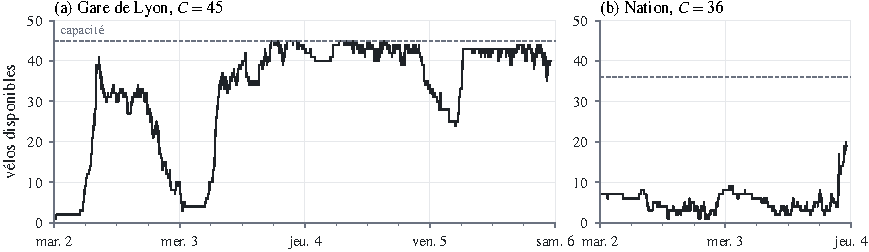
\includegraphics[width=\textwidth]{figures/fig_donnees.pdf}
\caption{Nombre de vélos disponibles, relevé chaque minute. (a)~Gare de Lyon, du mardi 2 au vendredi 5 juin 2026~; (b)~Nation, 2 et 3 juin. Tirets~: capacité.}\label{fig:donnees}
\end{figure*}

\begin{table}[t]
\centering\small
\caption{Séries utilisées. $\Nu$, $\Nd$~: dépôts et retraits comptés~; dernières colonnes~: minutes passées pleine et vide.}\label{tab:donnees}
\setlength{\tabcolsep}{4pt}
\begin{tabular}{@{}lrrrrrr@{}}
\toprule
Station & $C$ & heures & $\Nu$ & $\Nd$ & pleine & vide\\
\midrule
\multicolumn{7}{@{}l}{\emph{Jours ouvrés, 1\textsuperscript{er}--5 juin}}\\
\quad Gare de Lyon & 45 & 95{,}5 & 401 & 362 & 492 & 0\\
\quad Nation & 36 & 47{,}5 & 107 & 95 & 0 & 0\\
\multicolumn{7}{@{}l}{\emph{Week-end, 23--24 mai}}\\
\quad Gare de Lyon & 45 & 24{,}0 & 81 & 102 & 157 & 0\\
\quad Nation & 36 & 24{,}0 & 43 & 41 & 0 & 17\\
\quad Parc des Princes & 32 & 24{,}0 & 68 & 58 & 89 & 0\\
\quad Claude Terrasse & 46 & 24{,}0 & 84 & 74 & 82 & 0\\
\bottomrule
\end{tabular}
\end{table}

\subsection{Le régime stationnaire n'est pas observé}\label{sec:nonstationnaire}

Le TIPE ajustait le modèle à taux constants sur la journée du mardi, de 9~h à 19~h. On obtient $\hat\lambda=3{,}50$ $[2{,}51\,;\,4{,}87]$ et $\hat\mu=4{,}80$ $[3{,}62\,;\,6{,}37]\hr$, soit $\hat\rho=0{,}73$ $[0{,}47\,;\,1{,}13]$ (tableau~\ref{tab:fenetres}). La loi stationnaire place alors la station près de $0$~: $\EE_\pi[X]=2{,}7$, alors que la station contient en moyenne 30{,}6~vélos sur la fenêtre. La distance en variation totale entre $\pi$ et l'occupation observée vaut 0{,}999 (fig.~\ref{fig:stationnaire}a). Le TIPE concluait à l'échec du modèle.

C'est l'approximation stationnaire qui échoue, pas le modèle. La loi de $X_t$ issue de l'état observé à 9~h ($X=34$), calculée avec les mêmes taux, contient la trajectoire dans sa bande à 90~\% pendant 100~\% des minutes (fig.~\ref{fig:stationnaire}b). Le temps de relaxation vaut 8{,}2~h et le temps de mélange 33{,}3~h~: sur une fenêtre de 10~h, la chaîne n'a pas le temps d'oublier son état initial. À Nation, sur la même fenêtre, $\trel=29{,}5$~h et $\tmel=66{,}0$~h.

\begin{figure}[t]
\centering
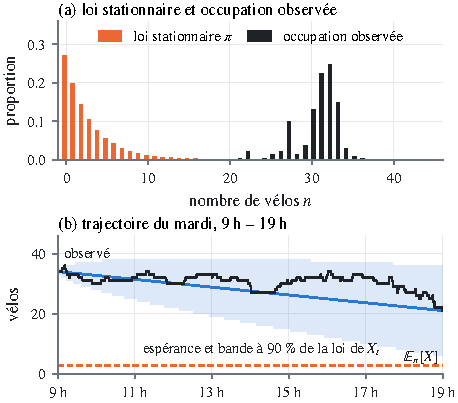
\includegraphics[width=\columnwidth]{figures/fig_stationnaire.pdf}
\caption{Gare de Lyon, mardi 2 juin, 9~h--19~h. (a)~Loi stationnaire du modèle ajusté ($\hat\rho=0{,}73$) et occupation observée. (b)~Trajectoire observée, espérance et bande à 90~\% de la loi de $X_t$ issue de l'état observé à 9~h, avec les mêmes taux.}\label{fig:stationnaire}
\end{figure}

\begin{table}[t]
\centering\small
\caption{Estimations sur quelques fenêtres, avec l'intervalle de confiance à 95~\% de $\rho$ (section~\ref{sec:estimation}). Taux en $\mathrm{h}^{-1}$.}\label{tab:fenetres}
\setlength{\tabcolsep}{3.5pt}
\begin{tabular}{@{}lrrrrl@{}}
\toprule
Fenêtre & $\Nu$ & $\Nd$ & $\hat\lambda$ & $\hat\mu$ & $\hat\rho$ \ [IC 95~\%]\\
\midrule
\multicolumn{6}{@{}l}{\emph{Gare de Lyon}}\\
\quad mardi 6--8~h & 27 & 1 & 13{,}5 & 0{,}50 & 27{,}0 \ [3{,}67\,;\,199]\\
\quad mercredi 6--8~h & 27 & 2 & 13{,}5 & 1{,}00 & 13{,}5 \ [3{,}21\,;\,56{,}8]\\
\quad mardi 9--19~h & 35 & 48 & 3{,}50 & 4{,}80 & 0{,}73 \ [0{,}47\,;\,1{,}13]\\
\quad mardi 18--20~h & 14 & 22 & 7{,}00 & 11{,}0 & 0{,}64 \ [0{,}33\,;\,1{,}24]\\
\quad 1\textsuperscript{er}--5 juin & 401 & 362 & 4{,}60 & 3{,}79 & 1{,}21 \ [1{,}05\,;\,1{,}40]\\
\quad 23--24 mai & 81 & 102 & 3{,}79 & 4{,}25 & 0{,}89 \ [0{,}67\,;\,1{,}19]\\
\multicolumn{6}{@{}l}{\emph{Nation}}\\
\quad mardi 9--19~h & 21 & 25 & 2{,}10 & 2{,}50 & 0{,}84 \ [0{,}47\,;\,1{,}50]\\
\quad 1\textsuperscript{er}--3 juin & 107 & 95 & 2{,}26 & 2{,}00 & 1{,}13 \ [0{,}85\,;\,1{,}48]\\
\bottomrule
\end{tabular}
\end{table}

\subsection{Saisonnalité intrajournalière}\label{sec:saison}

On découpe la journée en douze créneaux de 2~h et on estime $(\lambda_k,\mu_k)$ en regroupant les quatre jours ouvrés (fig.~\ref{fig:forcage}, tableau~\ref{tab:creneaux}). La pointe du matin, de 6~h à 8~h, compte 66 dépôts pour 4 retraits~: $\hat\rho\approx20$. La station reçoit alors les vélos des usagers qui rejoignent la gare ou les bureaux du quartier. Le dimanche 24 mai, cette pointe disparaît ($\hat\lambda=2{,}0\hr$ de 6~h à 8~h) et les dépôts culminent de 10~h à 12~h ($\hat\lambda=14{,}4\hr$).

Les tests du rapport de vraisemblance (section~\ref{sec:rv}) donnent~:
\begin{itemize}
\item taux constants sur la journée~: $W=157{,}6$ (11 degrés de liberté, $p=4\cdot10^{-28}$) pour les dépôts, $W=171{,}5$ ($p=6\cdot10^{-31}$) pour les retraits~;
\item taux constants de 8~h à 20~h~: $p=0{,}018$ et $p=2{,}5\cdot10^{-4}$~;
\item même profil chaque jour, créneau par créneau~: $p=3{,}4\cdot10^{-3}$ et $p=9{,}8\cdot10^{-5}$.
\end{itemize}
Les taux varient au cours de la journée, et le profil lui-même varie d'un jour à l'autre. Le second point annonce des bandes de prédiction trop étroites hors échantillon~: des taux moyens ne captent pas la variabilité entre jours.

Tous les temps de mélange du tableau~\ref{tab:creneaux} dépassent 5{,}1~h, soit plus du double de la durée d'un créneau~; de 8~h à 22~h, ils sont compris entre 27{,}9 et 48{,}2~h. La loi stationnaire d'un créneau n'est donc jamais atteinte. Seule la loi transitoire, propagée de créneau en créneau, a un sens. La figure~\ref{fig:melange} illustre les deux régimes de la remarque~\ref{rem:melange}. De 8~h à 10~h ($\hat\rho\approx1$), la convergence est lente et diffusive. De 6~h à 8~h ($\hat\rho\approx20$), $1/\gamma$ ne vaut que 10~min, mais la chaîne issue de $0$ reste à distance $1$ de $\pi$ pendant plusieurs heures, le temps de traverser la station.

\begin{figure}[t]
\centering
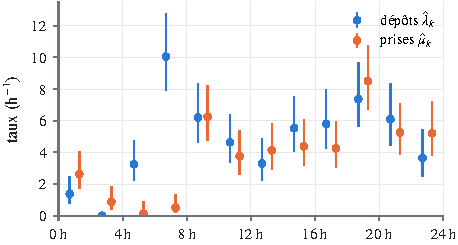
\includegraphics[width=\columnwidth]{figures/fig_forcage.pdf}
\caption{Taux de dépôt et de retrait par créneau de 2~h, Gare de Lyon, quatre jours ouvrés regroupés, avec intervalles de confiance à 95~\%.}\label{fig:forcage}
\end{figure}

\begin{table}[t]
\centering\small
\caption{Taux par créneau (en $\mathrm{h}^{-1}$), temps de relaxation et temps de mélange de la chaîne à taux constants correspondante, en heures. Aucun dépôt n'est observé de 2~h à 4~h.}\label{tab:creneaux}
\setlength{\tabcolsep}{4.5pt}
\begin{tabular}{@{}lrrrrr@{}}
\toprule
Créneau & $\hat\lambda_k$ & $\hat\mu_k$ & $\hat\rho_k$ & $\trel$ & $\tmel$\\
\midrule
0--2~h & 1{,}38 & 2{,}63 & 0{,}52 & 4{,}8 & 37{,}7\\
2--4~h & 0{,}00 & 0{,}88 & 0 & -- & --\\
4--6~h & 3{,}25 & 0{,}13 & 26{,}0 & 0{,}48 & 15{,}7\\
6--8~h & 10{,}05 & 0{,}50 & 20{,}1 & 0{,}16 & 5{,}1\\
8--10~h & 6{,}20 & 6{,}25 & 0{,}99 & 34{,}3 & 35{,}0\\
10--12~h & 4{,}63 & 3{,}75 & 1{,}24 & 15{,}1 & 44{,}3\\
12--14~h & 3{,}30 & 4{,}13 & 0{,}80 & 15{,}7 & 48{,}2\\
14--16~h & 5{,}53 & 4{,}38 & 1{,}26 & 11{,}0 & 35{,}0\\
16--18~h & 5{,}80 & 4{,}25 & 1{,}37 & 7{,}0 & 27{,}9\\
18--20~h & 7{,}36 & 8{,}50 & 0{,}87 & 12{,}8 & 29{,}2\\
20--22~h & 6{,}09 & 5{,}25 & 1{,}16 & 17{,}3 & 40{,}2\\
22--24~h & 3{,}65 & 5{,}21 & 0{,}70 & 6{,}3 & 28{,}3\\
\bottomrule
\end{tabular}
\end{table}

\begin{figure}[t]
\centering
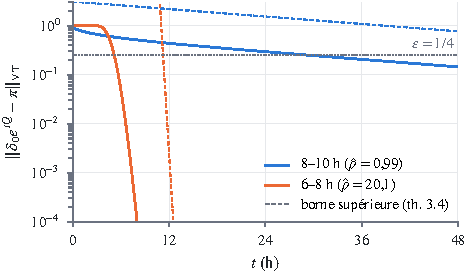
\includegraphics[width=\columnwidth]{figures/fig_melange.pdf}
\caption{Distance à l'équilibre depuis la station vide, avec les taux de deux créneaux de Gare de Lyon. Tirets~: majoration du théorème~\ref{thm:vitesse}~; pointillés~: seuil $1/4$ qui définit $\tmel$.}\label{fig:melange}
\end{figure}

\subsection{Prévision hors échantillon}\label{sec:prevision}

\paragraph{Protocole} Pour prévoir un jour, on estime les taux par créneau sur les autres jours ouvrés (validation croisée \og un jour exclu\fg{}), et on calcule la loi exacte de $X_t$ à partir de l'état observé au début de l'horizon. On mesure l'écart absolu moyen (EAM) entre l'espérance et la trajectoire, et la couverture de la bande à 90~\%, c'est-à-dire la fraction des minutes où la trajectoire est dans la bande.

\paragraph{Horizon 2~h} Sur les 47 créneaux de Gare de Lyon, la bande couvre 88{,}3~\% des minutes, pour 90~\% visés. En fin de créneau, la valeur observée sort de la bande 6 fois, contre 4{,}7 attendues (test binomial, $p=0{,}47$). L'erreur quadratique moyenne en fin de créneau vaut 4{,}6~vélos, contre 6{,}7 pour la prévision naïve \og pas de changement\fg{}. À Nation, station peu active, la couverture atteint 95{,}8~\%, mais la prévision naïve fait mieux (2{,}7 contre 3{,}3~vélos). Les trois créneaux les plus mal couverts, avec moins de 10~\% des minutes dans la bande, sont des nuits ou des soirées où la station perd des vélos, ce que les autres jours ne laissaient pas prévoir~: le mardi de 20~h à 22~h, elle passe de 20 à 11~vélos alors que l'espérance prévue monte à 26 (fig.~\ref{fig:court}b).

\begin{figure}[t]
\centering
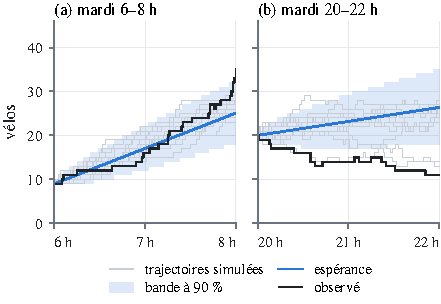
\includegraphics[width=\columnwidth]{figures/fig_court.pdf}
\caption{Prévision à 2~h hors échantillon, Gare de Lyon, mardi 2 juin~: taux estimés sur les trois autres jours, état initial observé. (a)~Pointe du matin~; (b)~soirée atypique.}\label{fig:court}
\end{figure}

\paragraph{Horizon 24~h} Le tableau~\ref{tab:jour} compare trois modèles partant de l'état observé à minuit~: taux constants et taux par créneaux, estimés hors échantillon, puis taux par créneaux estimés sur le jour même, en échantillon, qui donnent une borne inférieure de l'erreur. À Gare de Lyon, les créneaux réduisent l'EAM moyen de 8{,}5 à 5{,}5~vélos et portent la couverture de 73 à 86~\%. L'écart restant avec le modèle en échantillon (2{,}1~vélos) mesure la variabilité d'un jour à l'autre. Le mardi et le mercredi, qui démarrent presque vides, sont les plus mal prévus (fig.~\ref{fig:jour}).

\begin{table}[t]
\centering\small
\caption{Prévision à 24~h depuis l'état $X_0$ observé à minuit~: EAM en vélos et, entre parenthèses, couverture de la bande à 90~\% en pourcentage.}\label{tab:jour}
\setlength{\tabcolsep}{4pt}
\begin{tabular}{@{}lrlll@{}}
\toprule
Jour & $X_0$ & constants & créneaux & jour même\\
\midrule
\multicolumn{5}{@{}l}{\emph{Gare de Lyon}}\\
\quad mardi 2 & 1 & 10{,}2 (78) & 7{,}4 (84) & 1{,}8 (100)\\
\quad mercredi 3 & 10 & 17{,}4 (27) & 9{,}1 (73) & 1{,}8 (98)\\
\quad jeudi 4 & 43 & 2{,}2 (100) & 2{,}5 (100) & 1{,}6 (100)\\
\quad vendredi 5 & 34 & 4{,}1 (86) & 3{,}0 (88) & 3{,}1 (100)\\
\quad moyenne & & 8{,}5 (73) & 5{,}5 (86) & 2{,}1 (99)\\
\multicolumn{5}{@{}l}{\emph{Nation}}\\
\quad mardi 2 & 7 & 8{,}2 (92) & 3{,}6 (90) & 1{,}5 (100)\\
\quad mercredi 3 & 8 & 4{,}2 (100) & 2{,}2 (99) & 2{,}0 (100)\\
\quad moyenne & & 6{,}2 (96) & 2{,}9 (95) & 1{,}8 (100)\\
\bottomrule
\end{tabular}
\end{table}

\begin{figure*}[t]
\centering
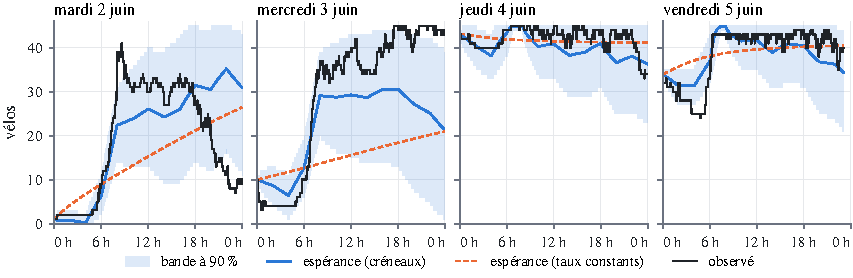
\includegraphics[width=\textwidth]{figures/fig_jour.pdf}
\caption{Prévision à 24~h hors échantillon depuis l'état observé à minuit, Gare de Lyon. Bleu~: taux par créneaux estimés sur les trois autres jours (espérance et bande à 90~\%)~; tirets orange~: taux constants.}\label{fig:jour}
\end{figure*}

\subsection{Régime périodique}\label{sec:regime}

En répétant chaque jour le profil moyen des taux, on se place dans le cadre de la proposition~\ref{prop:periodique}. La matrice $M$, produit des douze exponentielles, vérifie $|\lambda_2(M)|=0{,}13$ et $\delta(M)=0{,}65$~: l'écart à la loi invariante est divisé par environ 8 chaque jour. La loi invariante $\nu$ à minuit a pour moyenne 34{,}1~vélos et pour bande à 90~\% $[20\,;\,44]$~; sous $\nu$, $\PP(X\leq10)=0{,}007$. Le vélo unique du mardi 0~h et les 10 vélos du mercredi 0~h sont donc atypiques. Ils signalent une intervention extérieure, typiquement un camion de régulation, que le modèle ne contient pas.

La figure~\ref{fig:periodique} prolonge la prévision du mardi 0~h sur quatre jours. La distance en variation totale à $\nu$ passe de 0{,}34 à 24~h à 0{,}050 à 48~h, puis 0{,}007 à 72~h. La trajectoire reste dans la bande 98{,}8~\% du temps. La \og dérive\fg{} d'un jour à l'autre relevée dans le TIPE (le forçage se répète, pas la réponse) est ce régime transitoire~: la réponse se répète une fois l'état initial oublié, soit après deux jours environ.

\begin{figure*}[t]
\centering
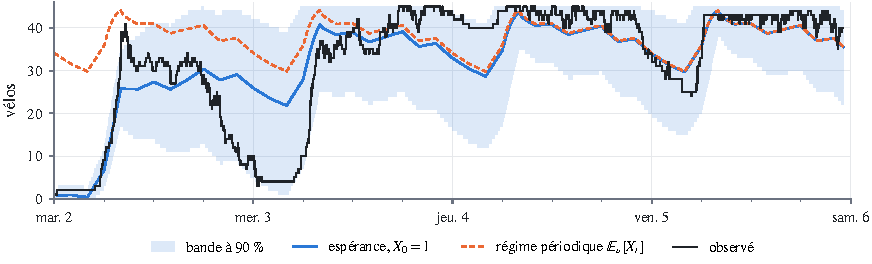
\includegraphics[width=\textwidth]{figures/fig_periodique.pdf}
\caption{Prévision sur quatre jours depuis le mardi 0~h ($X_0=1$), avec le profil moyen des taux répété chaque jour. Tirets~: espérance dans le régime périodique.}\label{fig:periodique}
\end{figure*}

\paragraph{Qualité de service} Dans le régime périodique, la station est pleine 13{,}9~\% du temps et refuse 19{,}9~\% des dépôts, fraction pondérée par l'intensité des dépôts (propriété PASTA)~; elle n'est presque jamais vide (0{,}03~\% du temps). Sur 4\,000 journées simulées à partir de $\nu$, la station sature au moins une fois dans 96{,}7~\% des cas~; le temps quotidien passé à saturation a pour médiane 194~min et pour intervalle à 90~\% $[22\,;\,392]$~min. Les valeurs observées du mardi au vendredi sont 0, 177, 222 et 93~min~; seule la première, après un départ presque vide, sort de l'intervalle.

\subsection{Écarts à l'hypothèse poissonnienne}\label{sec:poisson}

\paragraph{Arrivées groupées} Sous (H1), avec les taux du créneau, la variation nette d'une minute suit une loi de Skellam, différence de deux lois de Poisson indépendantes. Le tableau~\ref{tab:lots} compare le nombre de minutes où la station gagne, ou perd, au moins deux vélos au nombre attendu. Sur l'ensemble des séries, on observe 128 telles minutes pour 68{,}2 attendues, soit un facteur 1{,}9 ($p=7\cdot10^{-11}$ sous l'approximation de Poisson). Une partie des usagers arrive en groupe, par exemple à la descente d'un train à Gare de Lyon. Un processus de Poisson composé ou un processus de Hawkes \cite{BMM15} rendrait compte de cette surdispersion.

\begin{table}[t]
\centering\small
\caption{Minutes avec une hausse ($\Delta\geq2$) ou une baisse ($\Delta\leq-2$) d'au moins deux vélos~: nombre observé et nombre attendu sous (H1) avec les taux de chaque créneau.}\label{tab:lots}
\setlength{\tabcolsep}{4pt}
\begin{tabular}{@{}lrrrr@{}}
\toprule
& \multicolumn{2}{c}{$\Delta\geq2$} & \multicolumn{2}{c}{$\Delta\leq-2$}\\
\cmidrule(lr){2-3}\cmidrule(l){4-5}
Série & obs. & att. & obs. & att.\\
\midrule
\multicolumn{5}{@{}l}{\emph{Jours ouvrés}}\\
\quad Gare de Lyon & 35 & 23{,}0 & 29 & 15{,}1\\
\quad Nation & 7 & 3{,}4 & 3 & 2{,}2\\
\multicolumn{5}{@{}l}{\emph{Week-end}}\\
\quad Gare de Lyon & 9 & 5{,}0 & 10 & 5{,}3\\
\quad Nation & 6 & 0{,}8 & 1 & 0{,}8\\
\quad Parc des Princes & 9 & 2{,}4 & 2 & 1{,}6\\
\quad Claude Terrasse & 11 & 6{,}4 & 6 & 2{,}2\\
\midrule
Total & 77 & 41{,}0 & 51 & 27{,}2\\
\bottomrule
\end{tabular}
\end{table}

\paragraph{Régulation} Certaines variations sont incompatibles avec le modèle. À Nation, le mercredi 3 juin entre 21~h~36 et 21~h~46, la station passe de 4 à 17~vélos. Avec le taux de dépôt de la veille sur le même créneau ($2{,}0\hr$), la probabilité d'au moins 13 dépôts en 10~min est de l'ordre de $7\cdot10^{-17}$. À Gare de Lyon, le dimanche 24 mai à 20~h~54, la station perd 5~vélos en une minute ($p\approx9\cdot10^{-7}$ avec le taux de retrait du créneau précédent). Ce sont des camions de l'opérateur. La régulation est un contrôle exogène~: le modèle complet est une chaîne contrôlée, avec des sauts imposés à des instants choisis par l'opérateur.

\section{Discussion~: lecture en finance quantitative}\label{sec:discussion}

\paragraph{Files d'ordres} Dans le modèle de Cont, Stoikov et Talreja \cite{CST10}, la quantité d'ordres à chaque niveau de prix est un processus de naissance et de mort~: les ordres limites l'alimentent, les ordres au marché et les annulations la vident. La probabilité que le meilleur prix monte est celle qu'une file se vide avant une autre, un problème de premier passage du type du corollaire~\ref{cor:ruine}, résolu par transformée de Laplace. Cont et de Larrard \cite{CdL13} en tirent une limite diffusive du prix. Huang, Lehalle et Rosenbaum \cite{HLR15} font dépendre les intensités de la taille de la file. Pour une station, l'analogue serait des taux $\lambda(n)$ et $\mu(n)$ dépendant de $n$, par exemple si l'application détourne les usagers des stations presque vides. La loi stationnaire reste explicite par équilibre détaillé~: $\pi_n\propto\prod_{j=0}^{n-1}\lambda(j)/\mu(j+1)$.

\paragraph{Risque de crédit} Jarrow, Lando et Turnbull \cite{JLT97} décrivent la notation d'un émetteur par une chaîne de Markov à temps continu dont le défaut est l'état absorbant. Lando et Skødeberg \cite{LS02} estiment le générateur à partir des dates exactes de migration, avec l'estimateur de la proposition~\ref{prop:emv}~; l'estimateur en temps continu attribue une probabilité non nulle à des transitions rares jamais observées sur un an. La remarque de la section~\ref{sec:minute} sur la compensation en est la version à la minute~: l'échantillonnage discret masque les allers-retours, pas la dérive.

\paragraph{Saisonnalité et agrégats} L'intensité des transactions suit un profil intrajournalier marqué, que l'on traite comme ici par une intensité déterministe par morceaux avant de modéliser le résidu. Les arrivées groupées (section~\ref{sec:poisson}) et la variabilité entre jours (section~\ref{sec:saison}) ont pour analogues les agrégats d'ordres que décrivent les processus de Hawkes \cite{BMM15}.

\paragraph{Validation} Le protocole de la section~\ref{sec:prevision} est celui d'un backtest~: paramètres estimés sur une période, prévision évaluée sur une autre, couverture comparée au niveau nominal comme pour une VaR \cite{Kup95}. Les minutes successives étant très corrélées, le test porte sur les valeurs de fin de créneau.

\paragraph{Limites} Les données couvrent six jours~; les taux d'un créneau reposent sur quatre jours au plus, d'où des intervalles larges (fig.~\ref{fig:forcage}). Chaque station est traitée isolément, alors que les dépôts d'une station sont les retraits d'une autre. Les camions de régulation ne sont pas modélisés.

\section{Conclusion}

Une station Vélib' se décrit bien par une chaîne de naissance et de mort à taux constants par créneaux, à condition de calculer la loi transitoire et non la loi stationnaire. Les temps de mélange, de 5 à 48~h, dépassent la durée pendant laquelle les taux restent constants~: la loi stationnaire d'un créneau n'est jamais observée. L'objet pertinent est le régime périodique, atteint en deux jours environ. Hors échantillon, le modèle prévoit l'occupation à 2~h avec une couverture proche du niveau visé~; à 24~h, la variabilité entre jours domine. Les écarts restants, arrivées groupées et camions de régulation, indiquent les extensions naturelles~: processus de Poisson composé ou de Hawkes, intensités dépendant de l'état, contrôle optimal de la régulation.

\appendix
\section{Code}\label{sec:code}

Le module \texttt{velib.py} contient les fonctions de simulation, d'estimation et de calcul exact. Les scripts fournis avec l'article (lecture des relevés, calculs, figures) s'appuient sur ce module, sur \texttt{numpy}, \texttt{scipy} et \texttt{matplotlib}.

\begin{lstlisting}[style=py]
import numpy as np
from scipy.linalg import expm


# ---------- 1. Simulation ----------

def gillespie(C, lam, mu, duree, n0, rng):
    """Trajectoire a taux constants sur [0, duree]."""
    t = 0.0
    n = n0
    temps = [0.0]
    etats = [n0]
    while True:
        depot = lam if n < C else 0.0
        prise = mu if n > 0 else 0.0
        total = depot + prise
        if total == 0:
            break
        # delai avant le prochain evenement
        t = t + rng.exponential(1 / total)
        if t >= duree:
            break
        # nature de l'evenement
        if rng.random() < depot / total:
            n = n + 1
        else:
            n = n - 1
        temps.append(t)
        etats.append(n)
    return np.array(temps), np.array(etats)


def gillespie_creneaux(C, lam_tab, mu_tab, hc, n0, rng):
    """Taux constants sur des creneaux de duree hc."""
    temps = [0.0]
    etats = [n0]
    n = n0
    for k in range(len(lam_tab)):
        # simulation homogene sur le creneau k,
        # depuis l'etat atteint a la fin du precedent
        T, E = gillespie(C, lam_tab[k], mu_tab[k],
                         hc, n, rng)
        for j in range(1, len(T)):
            temps.append(k * hc + T[j])
            etats.append(E[j])
        n = E[-1]
    return np.array(temps), np.array(etats)


def echantillonner(temps, etats, grille):
    """Trajectoire lue aux instants de la grille."""
    valeurs = np.zeros(len(grille), dtype=int)
    j = 0
    for i in range(len(grille)):
        while (j + 1 < len(temps)
               and temps[j + 1] <= grille[i]):
            j = j + 1
        valeurs[i] = etats[j]
    return valeurs


# ---------- 2. Estimation ----------

def estimer_taux(velos, libres, pas=1 / 60):
    """Comptages et expositions (pas en heures)."""
    depots = 0
    prises = 0
    t_depot = 0.0   # temps ou un depot est possible
    t_prise = 0.0   # temps ou une prise est possible
    for i in range(len(velos) - 1):
        d = velos[i + 1] - velos[i]
        if d > 0:
            depots = depots + d
        if d < 0:
            prises = prises - d
        if libres[i] > 0:
            t_depot = t_depot + pas
        if velos[i] > 0:
            t_prise = t_prise + pas
    return depots, t_depot, prises, t_prise


def intervalle(nb, expo, z=1.96):
    """Taux estime et intervalle de confiance a 95 %."""
    taux = nb / expo
    marge = np.exp(z / np.sqrt(nb))
    return taux, taux / marge, taux * marge


# ---------- 3. Modele theorique ----------

def loi_stationnaire(C, lam, mu):
    rho = lam / mu
    poids = np.array([rho**n for n in range(C + 1)])
    return poids / poids.sum()


def generateur(C, lam, mu):
    Q = np.zeros((C + 1, C + 1))
    for n in range(C + 1):
        if n < C:
            Q[n, n + 1] = lam
        if n > 0:
            Q[n, n - 1] = mu
        Q[n, n] = -Q[n].sum()
    return Q


def trou_spectral(C, lam, mu):
    r = np.sqrt(lam * mu)
    return lam + mu - 2 * r * np.cos(np.pi / (C + 1))


def lois_par_minute(C, lam_tab, mu_tab, hc, n0):
    """Loi de X_t minute par minute (Kolmogorov)."""
    p = np.zeros(C + 1)
    p[n0] = 1.0
    lois = [p]
    for k in range(len(lam_tab)):
        Q = generateur(C, lam_tab[k], mu_tab[k])
        P = expm(Q / 60)      # transition sur une minute
        for i in range(round(60 * hc)):
            p = p @ P
            lois.append(p)
    return np.array(lois)


def quantile(loi, niveau):
    """Plus petit n tel que P(X <= n) >= niveau."""
    cumul = 0.0
    for n in range(len(loi)):
        cumul = cumul + loi[n]
        if cumul >= niveau:
            return n
    return len(loi) - 1


def temps_moyen_atteinte(Q, cible):
    """m(n) = E_n[T_cible] : Q m = -1 hors de la cible."""
    autres = [n for n in range(len(Q)) if n not in cible]
    A = Q[np.ix_(autres, autres)]
    m = np.zeros(len(Q))
    m[autres] = np.linalg.solve(A, -np.ones(len(autres)))
    return m
\end{lstlisting}

\begin{thebibliography}{STGH18}
\small\sloppy\NoAutoSpacing
\setlength{\itemsep}{1pt}
\bibitem[Alb62]{Alb62} A.~Albert. Estimating the infinitesimal generator of a continuous time, finite state Markov process. \emph{Ann. Math. Statist.}, 33(2):727--753, 1962.
\bibitem[Bil61]{Bil61} P.~Billingsley. \emph{Statistical Inference for Markov Processes}. University of Chicago Press, 1961.
\bibitem[BMM15]{BMM15} E.~Bacry, I.~Mastromatteo, J.-F.~Muzy. Hawkes processes in finance. \emph{Market Microstructure and Liquidity}, 1(1):1550005, 2015.
\bibitem[Bré99]{Bre99} P.~Brémaud. \emph{Markov Chains: Gibbs Fields, Monte Carlo Simulation, and Queues}. Springer, 1999.
\bibitem[CdL13]{CdL13} R.~Cont, A.~de Larrard. Price dynamics in a Markovian limit order market. \emph{SIAM J. Financial Math.}, 4(1):1--25, 2013.
\bibitem[CST10]{CST10} R.~Cont, S.~Stoikov, R.~Talreja. A stochastic model for order book dynamics. \emph{Oper. Res.}, 58(3):549--563, 2010.
\bibitem[DVJ03]{DVJ03} D.~J.~Daley, D.~Vere-Jones. \emph{An Introduction to the Theory of Point Processes}, vol.~I. Springer, 2\textsuperscript{e}~éd., 2003.
\bibitem[FG16]{FG16} C.~Fricker, N.~Gast. Incentives and redistribution in homogeneous bike-sharing systems with stations of finite capacity. \emph{EURO J. Transp. Logist.}, 5(3):261--291, 2016.
\bibitem[Gil77]{Gil77} D.~T.~Gillespie. Exact stochastic simulation of coupled chemical reactions. \emph{J. Phys. Chem.}, 81(25):2340--2361, 1977.
\bibitem[Guy07]{Guy07} A.~Guyader. \emph{Processus markoviens de sauts}. Notes de cours, master de statistique, Université Rennes~2, 2006--2007.
\bibitem[HLR15]{HLR15} W.~Huang, C.-A.~Lehalle, M.~Rosenbaum. Simulating and analyzing order book data: the queue-reactive model. \emph{J. Amer. Statist. Assoc.}, 110(509):107--122, 2015.
\bibitem[JLT97]{JLT97} R.~A.~Jarrow, D.~Lando, S.~M.~Turnbull. A Markov model for the term structure of credit risk spreads. \emph{Rev. Financ. Stud.}, 10(2):481--523, 1997.
\bibitem[JP04]{JP04} J.~Jacod, P.~Protter. \emph{Probability Essentials}. Springer, 2\textsuperscript{e}~éd., 2004.
\bibitem[Kup95]{Kup95} P.~H.~Kupiec. Techniques for verifying the accuracy of risk measurement models. \emph{J. Derivatives}, 3(2):73--84, 1995.
\bibitem[LP17]{LP17} D.~A.~Levin, Y.~Peres, avec E.~L.~Wilmer. \emph{Markov Chains and Mixing Times}. American Mathematical Society, 2\textsuperscript{e}~éd., 2017.
\bibitem[LS02]{LS02} D.~Lando, T.~M.~Skødeberg. Analyzing rating transitions and rating drift with continuous observations. \emph{J. Bank. Finance}, 26(2--3):423--444, 2002.
\bibitem[Nor97]{Nor97} J.~R.~Norris. \emph{Markov Chains}. Cambridge University Press, 1997.
\bibitem[RK13]{RK13} T.~Raviv, O.~Kolka. Optimal inventory management of a bike-sharing station. \emph{IIE Trans.}, 45(10):1077--1093, 2013.
\bibitem[SHH17]{SHH17} J.~Schuijbroek, R.~C.~Hampshire, W.-J.~van Hoeve. Inventory rebalancing and vehicle routing in bike sharing systems. \emph{European J. Oper. Res.}, 257(3):992--1004, 2017.
\bibitem[STGH18]{STGH18} J.~F.~Shortle, J.~M.~Thompson, D.~Gross, C.~M.~Harris. \emph{Fundamentals of Queueing Theory}. Wiley, 5\textsuperscript{e}~éd., 2018.
\bibitem[Wol82]{Wol82} R.~W.~Wolff. Poisson arrivals see time averages. \emph{Oper. Res.}, 30(2):223--231, 1982.
\end{thebibliography}

\end{document}
